%!TEX encoding = UTF-8 Unicode  
\documentclass{article}  
\usepackage{xeCJK}
\setCJKmainfont[BoldFont=STZhongsong, ItalicFont=STKaiti]{STSong}
\setCJKsansfont[BoldFont=STHeiti]{STXihei}
\setCJKmonofont{STFangsong}
\usepackage{graphicx}

\begin{document}  

\title{稀疏矩阵}
\date{}

\maketitle



就像在上一节描述的一样,标准的离散化的偏微分方程往往会伴随着一个庞大的且稀疏的矩阵。稀疏矩阵可以被模糊的描述为一个具有非常少的非零元的矩阵。但是,事实上,当特殊的技巧需要利用到大量的非零元以及它们的位置时,一个矩阵是可以被稀疏化的。这些稀疏化矩阵的技巧是从不储存零元的想法开始的。一个关键的问题是制定能够适合于高效地使用不论是直接还是迭代的标准计算方法的存储稀疏矩阵的数据结构。这一章节将简介稀疏矩阵,它们的属性、呈现,以及用以存储它们的数据结构。
\newline\newline

\textbf{3.1介绍}
\newline\newline
利用一个矩阵中的零元以及它们的位置的自然的想法最初是由在不同学科的工程师们提出的。在涉及带状矩阵的简单地例子中,特殊的技巧直接的被发明了。在20世纪60年代研发电子网络的电子工程师们是最早的去利用稀疏性来对于具有特殊结构的矩阵解决一般稀疏线性系统。对于稀疏矩阵技巧而言,最主要也是最早需要解决的问题是去设计一个在线性系统中得直接求解算法。这些算法需要是可以接受的,在存储和计算效率上。直接的稀疏算法可以被用于计算那些庞大的难以被稠密算法来实现的问题。
\newline\newline\newline\newline\newline\newline\newline\newline

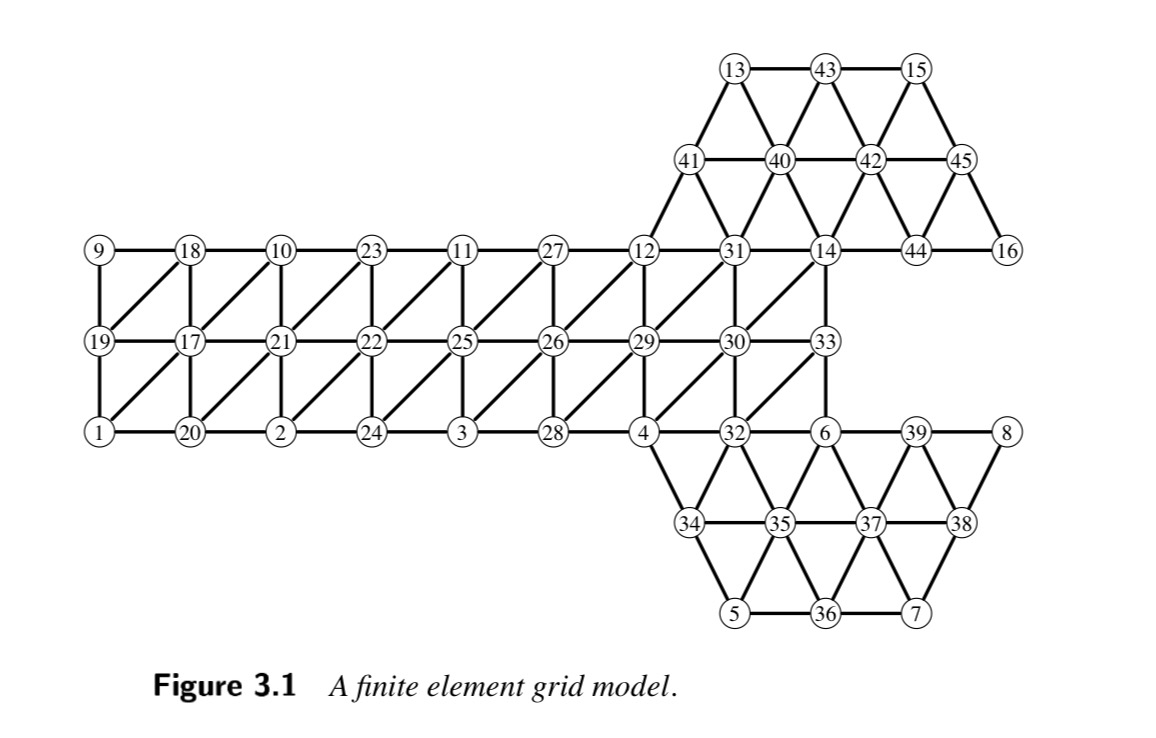
\includegraphics[scale=0.25]{3_1.png}

基本上,有两个明显的类别的稀疏矩阵,结构化的和非结构化的。一个结构化的矩阵是指一个非零元的位置形成某个规律的矩阵,通常这些非零元在对角线附近。要不然,这些非零元会在相同大小的块内(稠密子矩阵),而这也会形成一个规律,通常这些非零元在对角线(块)附近。一个具有着不规则位置的非零元的矩阵会被称作是非结构化的。最好的一个结构化的矩阵的例子是一个只有着少量对角元的矩阵。网格上的有限差分矩阵,就像上一节中提到的,是典型的具有着规律结构的例子。大部分的对于复杂几何的有限元和有限体积技巧会导致非结构化的矩阵。图3.2展示了一个与图3.1所呈现的有限元网格问题的一个小规模的非结构化的矩阵。
\newline

这两种类型的矩阵间的区别可能并不会明显的影响到直接求解技巧,而且,在过去,它并没受到过多的关注。但是,对于迭代求解方法,这个区别是很重要的。在这些方法中,最基本的运算之一是矩阵向量求积。在高性能计算机上,这些运算受规则化程度的影响很大。比如,在向量计算机上,理想的是存储对角元,但是更通常的设计可能会较慢,因为他们需要间接寻址。
\newline

下一节将讨论用图来呈现稀疏矩阵。
\newline\newline\newline\newline\newline\newline
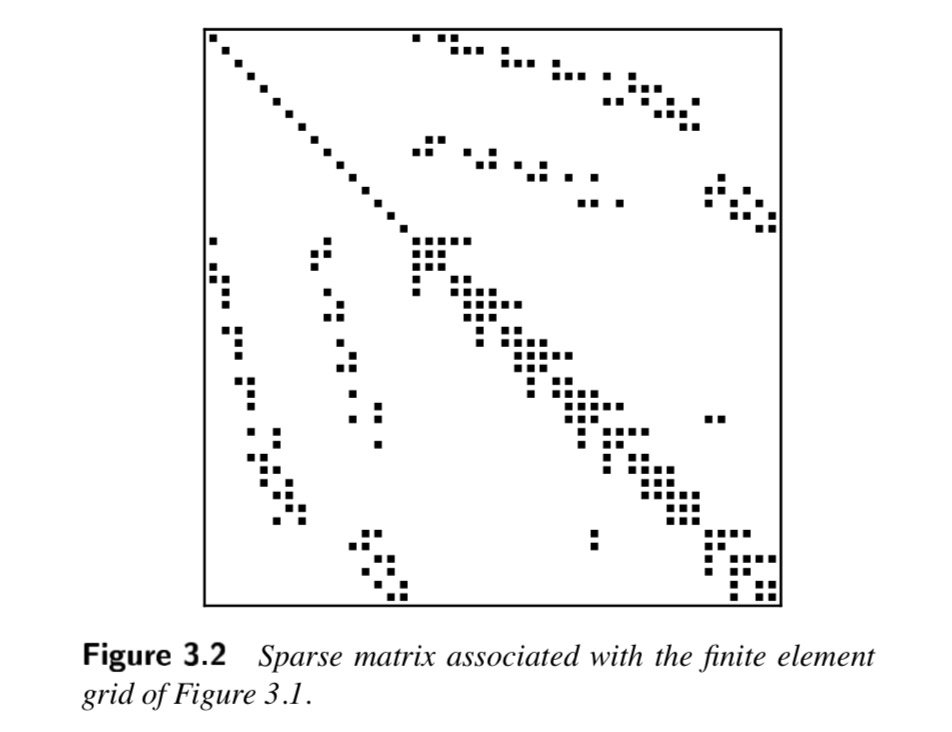
\includegraphics[scale=0.4]{3_2.png}
\newline\newline
\textbf{3.2图论}
\newline
图论是用来表示稀疏矩阵结构的一个理想的工具,因此,在稀疏矩阵技巧中,它扮演着一个主要的角色。例如,图论是用于解决并行稀疏高斯消除和预处理技术的关键。在下一节中,将讨论图的一般特性,以及它们在有限元和有限差分矩阵中得应用。
\newline
\textbf{3.2.1图与邻接图}
记住一个图由两个集合定义,一个顶点集合$V =\{v_1,v_2,\cdots,v_n\}$和一个边的集合E,E是由点对$(v_i,v_j)$组成的,$v_i,v_j$都是V中的元素,换而言之,$E\subseteq V\times V$。这个图$G=(V,E)$通常被平面内的一系列的被边联系的点的向量来表示。这个图被用来描述集合V中元素间的关系。例如,V可以被用来描述世界上的主要城市。线就是两个城市间的直达航线。那么这个图就会描述这样一个关系“在城市A和城市B间存在一条直达航线”。在这个特殊的例子中,二元关系很可能是对称的,换而言之,如果有一条A到B的直达航线,那么也有一条B到A的直达航线。在这样的情形中,图被称作是无向的,用以与通常的有向图相对。
  \newline\newline\newline\newline\newline\newline
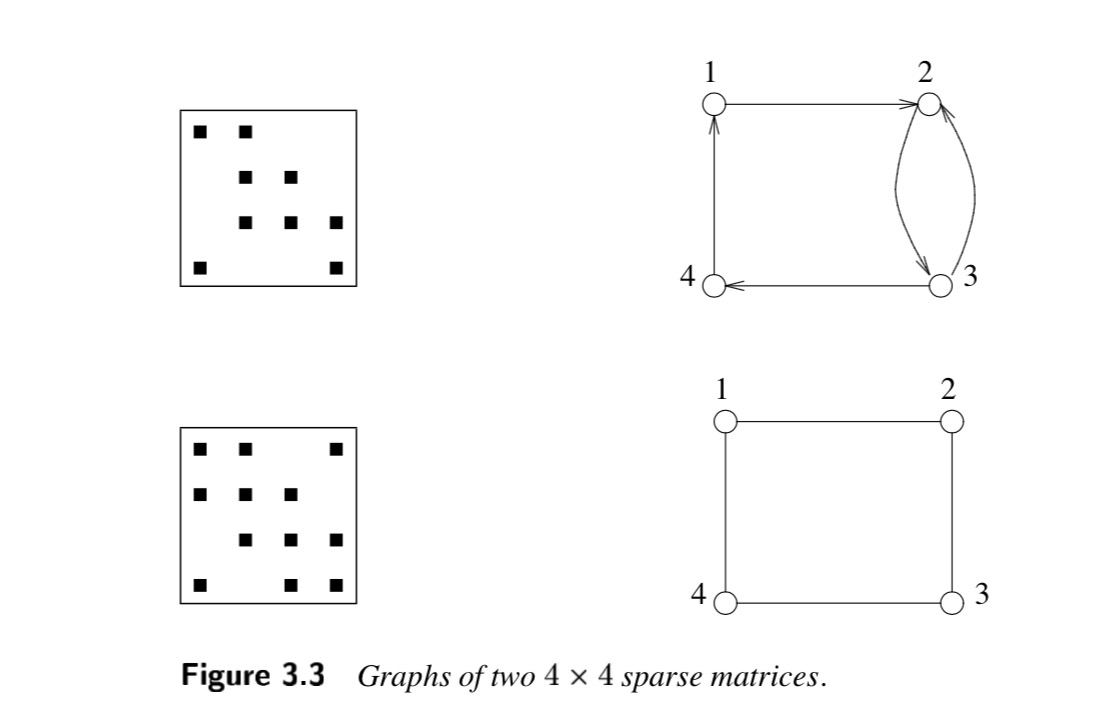
\includegraphics[scale=0.25]{3_3.png}
\newline\newline
回到稀疏矩阵,稀疏矩阵的邻接图是一个图$G=(V,E)$,V中得n个顶点代表n个未知数。它的边是按照以下规则建立的方程式建立的二元关系:当$a_{ji}\neq0$时,有一条从节点i指向节点j的边。而这条边将因此描述包含未知量j的二元关系方程式i。注意,这个图是有向的,除非这个矩阵是有对称结构的(对任意的$1\leq i,j\leq n$,若$a_{ji}\neq 0$,那么$a_{ij}\neq 0$ )。
\newline
当一个矩阵的非零元总有一个对称非零元,换而言之$a_{ij}$和$a_{ji}$总是同时为非零元,那么这图就是无向的。因此,对于无向图,每条边都有两个方向。因此,无向图可以用无向边来表现。
\newline
作为利用图模型的例子,并行高斯消去法可以通过寻找在指定消去阶段的未知数来获得。根据以上的二元关系,这些未知数两两独立。这些与未知数一致的行可以被用作基。因此,在一个极端情况下,当一个矩阵是对角阵,那么所有的未知数是独立的。与之相反的是,当一个矩阵是稠密的,那么每一个未知量都与其他未知量相关。稀疏矩阵则介于这两种极端情况之间。
\newline
邻接图有一些有趣的简单性质。$A^2$的图可以被解释成一个n顶点图,对每条边的点对(i,j), 表示在原图A中至少存在一条长度确切的说是2的从节点i到节点j的路径。与之相似的时,$A^k$的图包含的时用以描述从节点i到节点j的至少存在一条长度为k的路径的二元关系的边。欲知详情,请看练习4.
\newline
\textbf{3.2.2PDE矩阵的图}
\newline
对于在每个网格点只涉及一个屋里未知量的偏微分方程,离散矩阵的邻接图通常就是用来描述网格的图。但是,在每个网格点上有着多个未知量是很常见的。例如,模拟流体流动的方程可能涉及流体的两个速度分量(二维)以及在每个网格点的能量和动量。在这样的情况下,有两种用来标记未知量的选择。在每个网格点,它们可以被连续的标记。因此,在刚才的例子中,我们可以在一个指定的网格点例如u(k),$\cdots$,u(k+3)上标记所有的四个未知量(两个速度的分量,动量以及压力)。另外,所有的与一类变量相关的未知量可以最先被标记(比如,第一个速度分量),接下来是第二类的变量(比如,第二个速度分量)等等。在任意情况下,很明显邻接矩阵是有冗余信息的。物理网格的商图可以被用来替代使用。这将节约大量的存储量和计算量。在上述的流体流动的例子中,用以描述图的整数数组的存储可以被缩小到接近1/16。这是因为边的数量被所见到了大约这么多,但是通常很小的顶点数却保持着不变。
\newline
\textbf{3.3置换和重新排序}
\newline

\end{document}  
